\chapter{Grundlagen der Topologie}\label{chap:topologie-grundlagen}

Die in der vorliegenden Arbeit angegebenen Strukturen bauen auf topologischen Begriffen auf.
Die Abschnitte \ref{sec:allg-top-raeume} (Allgemeine topologische Räume), \ref{sec:teilraum-top} (Teilraumtopologie) und \ref{sec:top-metr-raeume} (Metrische Räume) führen Grundbegriffe der Topologie ein, wie sie auch in der Literatur zu finden sind. Sie dienen in erster Linie dazu die hier verwendeten Notationen einzuführen enthalten aber auch einige Sätze und Beweise.

Die eingeführten Begriffe und Notationen finden sich auf den herausnehmbaren Übersichtsblättern (Übersicht 4).

%%% Allgemeine topologische Räume %%%%%%%%%%%%%%%%%%%%%%%%%%%%%%%%%%%%%%%%%%%%%%%%%%%%%%%


\section{Allgemeine topologische Räume}\label{sec:allg-top-raeume} 
    %
    In diesem Abschnitt werden grundlegende Begriffe der Topologie eingeführt sowie einige relevante Sätze vorgestellt. 
    Für ein tieferes Verständnis sei auf die Literatur verwiesen ([\cite{jaenich-k-2013--a}] oder [\cite{manetti-m-2015--a}]). 
    Für mich geht es hier vor allem darum, eigene Notationen einzuführen, da sich die Standardnotationen schnell als unpraktisch erweisen, wenn es nötig wird mit verschiedenen topologischen Räumen gleichzeitig zu arbeiten.
    
    Der
    %\marginpar{Topologischer Raum,\\Topologie,\\offene Menge}
    \marginpar{Topologischer Raum}
    grundlegendste Begriff hierbei ist natürlich der des topologischen Raumes.
    Das ist eine Menge, von der wir wissen, welche ihrer Teilmengen offen sind.
    \begin{dfn}[Topologischer Raum, Topologie, offene Menge]\label{def:top} \ \\
        Ein \thmemph{topologischer Raum} ist ein Paar $(X,\offen)$ bestehend aus
    %
        \begin{itemize}
            \item einer Menge $X$ (\thmemph{Grundmenge}) 
            \item einer Menge $\offen \subseteq 2^X$ von Teilmengen von $X$ (\thmemph{Topologie})
        \end{itemize}
    %
        mit folgenden Eigenschaften:
    %
        \begin{enumerate}
            \item[T1] $\varnothing, X \in \offen$ %($\O$ und $X$ sind offen) 
            \item[T2] $A,B \in \offen \quad \quad \Leftrightarrow \quad \quad A \cap B \in \offen$ %(und damit: endliche Schnitte offener Mengen sind offen)
            \item[T3] $\mathcal{A} \subseteq \offen \quad \quad \Rightarrow \quad \quad \bigcup\limits_{A \in \mathcal{A}} A \in \offen$ %(Beliebige Vereinigungen offener Mengen sind offen).
        \end{enumerate}
    %	
        Wenn $A \in \offen$ ist, so sagen wir: $A$ ist \thmemph{offen} in $(X, \offen)$.
    %
    \end{dfn}
    
    \begin{konv}\label{konv:top}
        Wenn wir schreiben \glqq Sei $X$ ein topologischer Raum\grqq , so ist der topologische Raum $(X, \offen_X)$ mit $X$ als Grundmenge und zugehöriger Topologie $\offen_X$ gemeint. Wenn keine Verwechslungsgefahr besteht, schreiben wir auch $\offen$ für $\offen_X$.
    \end{konv}
    
    Aus
    \marginpar{Standardtopologie auf $\R$}
    der Schule ist für die reellen Zahlen der Begriff des offenen Intervalls bekannt. Diese bilden für sich genommen jedoch noch keine Topologie, da Vereinigungen offener Intervalle, die sich nicht überschneiden, keine offene Intervalle sind.
    Durch Abschlussbildung unter Vereinigung lässt sich jedoch mit ihrer Hilfe eine Topologie definieren, die sogenannte Standardtopologie auf $\R$.
    
    \begin{bsp}[Standardtopologie auf $\R$]\label{bsp:standard-r}\ \\
        Auf $\R$ ist die Standardtopologie folgendermaßen definiert:\\
        Eine Menge $M \subseteq \R$ ist offen, wenn sie leer ist oder sich als Vereinigung offener Intervalle schreiben lässt.
    \end{bsp}
    In Abschnitt \ref{sec:top-metr-raeume} werden wir sehen, dass sich diese Topologie auch aus der Standardmetrik auf $\R$ ergibt.

    Eine
%     \marginpar{offene Umgebung,\\$\offen_X(p)$}
    \marginpar{offene Umgebung}
    offene Umgebung eines Punktes ist eine offene Menge, die ihn enthält.
    \begin{dfn}[Offene Umgebung, $\offen_X(p)$]\label{def:umg} \ \\
        Sei $X$ ein topologischer Raum. Eine Menge $U \subseteq X$ heißt \thmemph{offene Umgebung} von $p$ in $X$, wenn $p \in U \in \offen_X$ gilt. Die \thmemph{Menge der offenen Umgebungen} von $p$ in $X$ notieren wir mit $\offen_X(p)$. Falls wir nur eine Topologie betrachten, schreiben wir auch $\offen(p)$ für $\offen_X(p)$.
    \end{dfn}

    Abgeschlossene
%     \marginpar{abgeschlossene Menge,\\$\abg_X$}
    \marginpar{abgeschlossene Menge}
    Mengen sind Komplemente offener Mengen.
    \begin{dfn}[Abgeschlossene Menge, $\abg_X$] \label{def:CX} \ \\
        Seien $X$ ein topologischer Raum, $A \subseteq X$.
        $A$ heißt \thmemph{abgeschlossen} in $X$, falls $X \setminus A \in \offen_X$ ist.
        Die \thmemph{Menge der abgeschlossenen Mengen} in $X$ bezeichnen wir mit $\abg_X$ bzw. falls keine Verwechslungsgefahr besteht mit $\abg$.
    \end{dfn}
    Analog zur Angabe der offenen Mengen, könnten wir auch die abgeschlossenen Mengen nutzen, um eine Topologie zu charakterisieren. Genauer gesagt: Jedes Mengensystem mit den folgenden Eigenschaften charakterisiert eine Topologie.

    \begin{satz}[Eigenschaften der Menge $\abg$]\label{satz:CX}\ \\
        Sei $X$ ein topologischer Raum. Dann gelten
        \begin{enumerate}
            \item $\varnothing, X \in \abg$ 
            \item $A,B \in \abg \quad \quad \Rightarrow \quad \quad  A \cup B \in \abg$ 
            \item $\mathcal{A} \subseteq \abg \quad \quad \Rightarrow \quad \quad \bigcap\limits_{A \in \mathcal{A}} A \in \abg$ 
        \end{enumerate}
        (Beweis trivial)
    \end{satz}
%     (Beweis trivial)
    
    Folgender Satz ist eine einfache Folgerung aus den Definitionen.
    \begin{satz}\label{satz:differenz}%verwendung: satz:rand-abg
        Sei $X$ ein topologischer Raum, $A\in \abg$ und $B \in \offen$. Dann gelten:
        \begin{enumerate}
            \item $A \setminus B \in \abg$
            \item $B \setminus A \in \offen$
        \end{enumerate}    
    \end{satz}
    
    \begin{bew}
        Mit $A \in \abg$ ist $X\setminus A \in \offen$ und somit gelten
        \begin{enumerate}
            \item $X \setminus (A \setminus B) = (X \setminus A) \cup (X \cap B) \in \offen$.
            \item $B \setminus A = B \cap (X \setminus A) \in \offen$.
        \end{enumerate}
    \end{bew}


    Ein
%     \marginpar{Randpunkt,\\Randoperator,\\Rand,\\$\rand_X$}
    \marginpar{Rand}
    Randpunkt einer Menge ist ein Punkt, für den in jeder offenen Umgebung sowohl Punkte im Inneren als auch außerhalb der Menge liegen. Der Randoperator ordnet jeder Menge die Menge ihrer Randpunkte zu.

    \begin{dfn}[Randoperator] \label{def:rand} \ \\
        Sei $X$ ein topologischer Raum. Dann ist der \thmemph{Randoperator} $\rand_X : 2^X \rightarrow 2^X$ auf $X$ definiert durch:
    %	
        \begin{align*}
            \rand_X(A) := \{&x \in X \mid \forall\: U \in \offen_X(x) :\\ 
            &(\: U \cap A \neq \varnothing \:\land\: U \setminus A \neq \varnothing \:))\}
        \end{align*}
        
    \end{dfn}

    
    \begin{konv}
        Statt $\rand_X(A)$ schreiben wir auch $\rand_X A$ und falls keine Verwechslungsgefahr besteht $\rand(A)$ bzw. $\rand A$.
    \end{konv}

    
    Folgendes
    \marginpar{Standardbeispiel}
    Beispiel für den Rand einer Menge wird im Laufe der Arbeit immer wieder genutzt, um verschiedene Begriffe und Fälle zu verdeutlichen und 
    %im Abschnitt \ref{sssec:standardbsp} 
    im nächsten Kapitel ausgiebiger untersucht.
    Deshalb nenne ich es Standardbeispiel.
    Dies ist natürlich nicht vergleichbar mit der bereits erwähnten Standardtopologie oder der weiter unten eingeführten Standardmetrik, die auch außerhalb der vorliegenden Arbeit eine Bedeutung haben.
    
    \begin{bsp}[Standardbeispiel]\label{bsp:standardbsp}\ \\
        Sei $$A := \bigcup_{n \in \N} [2^{-2n}, 2^{-2n+1}]$$ aus dem mit der in Bsp.\ \ref{bsp:standard-r} definierten Standardtopologie versehenen Raum $\R$.
        Dann ist
        \begin{align*}
            \rand A = \{\frac{1}{2^n} \mid n \in \N\} \cup \{0\}
        \end{align*}
    \end{bsp}
    %\todo[inline]{BH: begründen? $\to$ FL: Nein, eigentlich nicht nötig, sondern gut einsehbar.\\
% 		Gestolpert bin ich darüber, dass ich zuerst von $\N$ inkl.\ 0 ausging und 
% 		$A := \bigcup_{n \in \N} [2^{-2n-2}, 2^{-2n-1}]$ vorschlagen wollte;
% 		mit $\N$ ohne 0 müsste es das ergänzte `$-$' im Exponenten der 2.\ Komponente aber lösen.
% 		An $\rand A$ lässt sich letztlich auch ersehen, wie $\N$ hier ausgelegt wird,
% 		daher muss m.E. auch kein Zusatzhinweis sein.
% 		}
    
    \begin{figure}[ht]
        \centering
        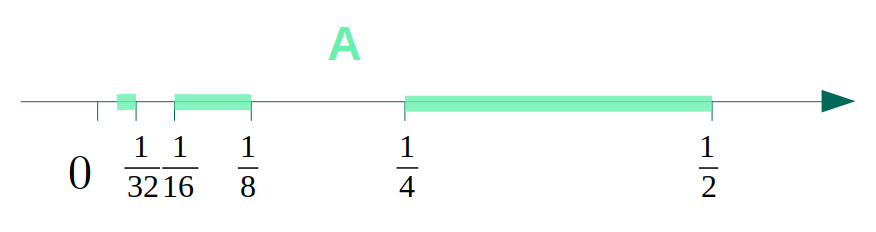
\includegraphics[width=0.6\textwidth]{abb/standardbsp.png}
        \caption{Zum Standardbeispiel}
        \label{fig:standardbsp}
    \end{figure}
    
    
    Der
%     \marginpar{Abschlussoperator,\\Abschluss,\\$\abg_X$}
    \marginpar{Abschluss}
    Abschluss einer Menge besteht aus der Menge selbst und all ihren Randpunkten. Diese Punkte liegen in dem Sinne \glqq sehr nah\grqq\ an der Menge, dass sie sich nicht durch offene Umgebungen von der Menge trennen lassen.
    
    \begin{dfn}[Abschlussoperator, Abschluss]\label{def:abschl} \ \\
        Sei $X$ ein topologischer Raum. Dann ist der \thmemph{Abschlussoperator} $\cl_X : 2^X \rightarrow 2^X$ auf $X$ definiert durch:
    %		
        \begin{align*}
            \cl_X(A) := \{x \in X \mid \forall\: U \in \offen_X(x) : U \cap A \neq \varnothing \}
        \end{align*}
    %	
        $\cl_X(A)$ heißt der \thmemph{Abschluss} von $A$.
    %	
    \end{dfn}
    %
    \begin{konv}
        Statt $\cl_X(A)$ schreiben wir auch $\cl(A)$ wenn klar ist, auf welche Topologie wir uns beziehen.
    \end{konv}
    
    \begin{bem}[Abschluss einer Menge unter einem Operator]\ \\
        Dem aufmerksamen Leser ist vielleicht aufgefallen, dass der Begriff des Abschlusses einer Menge in dieser Arbeit überladen ist.
        In Beispiel \ref{bsp:standard-r} wurde die Standardtopologie auf $\R$ als Abschluss der Menge der offenen Intervalle unter Vereinigung eingeführt.
        In Abschnitt \ref{sec:offene-fragen} wird die Frage aufgeworfen, ob sich ein Modell für $\theoryBSO$ durch Abschluss unter mereologischer Summenbildung zu einem Modell für $\theoryBS$ erweitern lässt.
        
        Diese beiden Beispiele benutzen den Begriff des Abschlusses einer Menge unter einem Operator. Formal:
        
        Sei $X$ eine Menge und $f: X^n \to X$ ein Operator auf $X$.
        Eine Menge $M \subseteq X$ ist \thmemph{abgeschlossen} unter $f$, falls für alle $m_1, ... , m_n \in M$ gilt: $f(m_1, ... m_n) \in M$.
        Der \thmemph{Abschluss} einer Menge $M$ unter einer Operation $f$ ist die kleinste unter $f$ abgeschlossene Menge, die $M$ enthält.
    \end{bem}


    Das
    \marginpar{Kern}
    Innere einer Menge besteht aus allen Punkten dieser Menge, die keine Randpunkte sind. Das bedeutet, diese Punkte haben offene Umgebungen, die komplett in der Menge liegen.

    \begin{dfn}[Kernoperator, Inneres] \label{def:kern} \ \\
        Sei $X$ ein topologischer Raum. Dann ist der \thmemph{Kernoperator} $\op_X : 2^X \rightarrow 2^X$ auf $X$ definiert durch:
    %	
        \begin{align*}
            \op_X(A) := \{x \in X \mid \exists \, U \in \offen_X(x) : U \subseteq A \}
        \end{align*}
    %	
        $\op_X(A)$ heißt das \thmemph{Innere} oder der \thmemph{Kern} von $A$.

    \end{dfn}

    \begin{konv}
        Statt $\op_X(A)$ schreiben wir auch $\op(A)$ wenn klar ist, auf welche Topologie wir uns beziehen.
    \end{konv}

    \begin{figure}[ht]
        \centering
        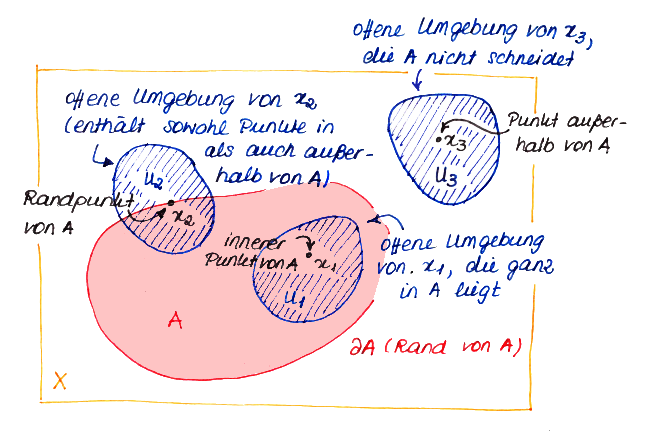
\includegraphics[height=7cm]{abb/top-grundbegr.png}
        \caption{Grundbegriffe der Topologie}
        \label{fig:top-grundbegr}
    \end{figure}


    \begin{bem}
        Üblicherweise werden der Abschluss von $A$ mit $\bar A$, das Innere mit $A^\circ$ bezeichnet. Da diese Notationen jedoch keine Unterscheidung zwischen verschiedenen Topologien zulassen, sind sie für die vorliegende Arbeit unpraktisch.
    \end{bem}
    
    \begin{bsp}[Abschluss und Kern am Standardbeispiel]\label{bsp:standardbsp-abschl-kern}\ \\
        Für die in Bsp.\ \ref{bsp:standardbsp} definierte Menge ${A = \bigcup_{n \in \N} [2^{-2n}, 2^{-2n+1}]}$ mit Rand\\${\rand A = \{\frac{1}{2^n} \mid n \in \N\} \cup \{0\}}$ sind Abschluss und Kern gegeben durch:
        \begin{align*}
            \cl(A) &= A \cup \rand A = A \cup \{0\}\\
            \op(A) &= A \setminus \rand A = \bigcup_{n \in \N} (2^{-2n}, 2^{-2n+1})
        \end{align*}
    \end{bsp}
%    \todo[inline]{BH: beweisen? $\to$ FL: Nein, danke, hinreichend einsehbar.\\
%		NB: Da ich hier erneut den Exponenten der 2.\ Komponente angepasst habe, wäre
%		ggf.\ die Arbeit nochmal an anderen Stellen des Standardbeispiels anzuschauen,
%		ob der Exponent auftritt.}

    Im
    \marginpar{Eigenschaften\\ von $\cl$, $\op$ und $\rand$}
    Folgenden werden hilfreiche Eigenschaften der topologischen Operatoren aufgeführt, die für die Beweise über die \strukt nützlich sind oder sein könnten.
    \begin{satz}[Eigenschaften des Abschlussoperators] \label{satz:cl}\ \\
        Sei $X$ ein topologischer Raum, $A, B \subseteq X$. Dann gelten
    %	
        \begin{enumerate}
            \item \label{satz:cl.1} $\cl(A)$ ist die kleinste in $X$ abgeschlossene Obermenge von $A$.
            \item \label{satz:cl.2} $\cl(A) = A \cup \rand(A)$.
            \item \label{satz:cl.3} $\cl(A \cap B) \subseteq \cl(A) \cap \cl(B)$
            \item \label{satz:cl.4} $\cl(A \cup B) = \cl(A) \cup \cl(B)$.
            \item \label{satz:cl.5} $\cl(X \setminus A) = X \setminus \op(A)$. 
            \item \label{satz:cl.6} $\cl(A \setminus B) \subseteq \cl(A) \setminus \op(B)$. 
            \item \label{satz:cl.7} $\cl(A) \setminus \cl(B) \subseteq \cl(A \setminus B)$
            \item \label{satz:cl.8} $A \subseteq B \quad \quad \Rightarrow \quad \quad \cl(A) \subseteq \cl(B)$ 
        \end{enumerate}	
        
    \end{satz}

    \begin{bew}%[Satz \ref{satz:cl}]
        \ 

        \noindent
        \thmemph{Zu \ref{satz:cl.1}:}
        Seien
        \begin{align} \label{mac}
            \mathcal{M}_A^C &:= \{ U \in \offen \mid U \cap A = \varnothing\} \\
            U_A^C &:= \bigcup\limits_{U \in \mathcal{M}_A^C} U
        \end{align}
        Dann ist $U_A^C$ als Vereinigung offener Mengen wieder offen und es gilt 
        \begin{align}
            \cl(A) = X \setminus U_A^C
        \end{align}
        (Beweis siehe Anhang \ref{anh:cl.1})\\
        Somit ist $\cl(A)$ als Komplement einer offenen Menge abgeschlossen. 
        Es bleibt noch zu zeigen, dass
        \begin{enumerate}
            \item $\cl(A)$ eine Obermenge von $A$ ist und
            \item es keine kleinere in $X$ abgeschlossene Menge gibt, die $A$ enthält.
        \end{enumerate}	 
        Auch diese Beweise sind im Anhang zu finden (ebenfalls \ref{anh:cl.1}).
        \\
            
        \noindent
        \thmemph{Zu \ref{satz:cl.2}-\ref{satz:cl.8}:} siehe \ref{anh:cl.2} - \ref{anh:cl.8}.

    \end{bew}


    \begin{kor} \label{kor:cl}\ \vspace{0pt}
        \begin{enumerate}
            \item \label{kor:cl.1} $\cl(A)$ ist abgeschlossen in X.
            \item \label{kor:cl.2} $A \subseteq \cl(A)$
            \item \label{kor:cl.3} $A \in \abg \quad \quad \Rightarrow \quad \quad \cl(A) = A$
            \item \label{kor:cl.4} $\cl(\cl(A)) = \cl(A)$
        \end{enumerate}
    \end{kor}

    \begin{bew}
        \

        \noindent 
        \thmemph{Zu \ref{kor:cl.1} und \ref{kor:cl.2}:} Offensichtliche Folgerungen aus Satz \ref{satz:cl}.		\ref{satz:cl.1}

        \noindent
        \thmemph{Zu \ref{kor:cl.4}:} Ebenfalls eine Folgerung aus Satz \ref{satz:cl}.\ref{satz:cl.1}. Dieser Satz besagt $\cl(\cl(A))$ ist die kleinste abgeschlossene Obermenge von $\cl(A)$. Da $\cl(A)$ selbst abgeschlossen ist (\ref{kor:cl.1}.) muss also gelten $\cl(\cl(A)) = \cl(A)$.

    \end{bew}


    \begin{satz}[Eigenschaften des Kernoperators] \label{satz:op}\ \\
        Sei $X$ ein topologischer Raum, $A, B \subseteq X$. Dann gelten:
    %	
        \begin{enumerate}
            \item \label{satz:op.1} $\op(A)$ ist die größte offene Teilmenge von A. %Verwendung: {satz:offeneMengenInAundKompl}
            \item \label{satz:op.2} $\op(A) = A \setminus \rand(A)$.
            \item \label{satz:op.3} $\op(A \cap B) = \op(A) \cap \op(B)$.
            \item \label{satz:op.4} $\op(A) \cup \op(B) \subseteq \op(A \cup B)$
            \item \label{satz:op.5} $\op(X \setminus A) = X \setminus \cl(A)$.
            \item \label{satz:op.6} $\op(A \setminus B) = \op(A) \setminus \cl(B)$. 
            \item \label{satz:op.7} $A \subseteq B \quad \Rightarrow \quad \op(A) \subseteq \op(B)$	
        \end{enumerate}	
        
    \end{satz}

    \begin{bew} 
    \ 

    \noindent
    \thmemph{Zu \ref{satz:op.1}:} Sei
        \begin{align}
            \mathcal{M}_A := \{U \in \offen \mid U \subseteq A\}.		
        \end{align}
        Dann gilt 
        \begin{align}
            \op(A) = \bigcup\limits_{U \in \mathcal{M}_A} U
        \end{align}
        (Beweis siehe Anhang \ref{anh:op.1})\\ 
        Dann ist $\op(A)$ als Vereinigung offener Mengen offen und als Vereinigung von Teilmengen von $A$ wieder eine Teilmenge von $A$. Außerdem gilt nach Konstruktion von $\mathcal{M}_A$
        \begin{align}
            \forall\: U \in \offen : U \subseteq A \rightarrow U \subseteq \op(A).
        \end{align}
        Damit ist also $\op(A)$ die größte offene Teilmenge von $A$.
        \\

        \noindent
        \thmemph{Zu \ref{satz:op.2}-\ref{satz:op.6}:} siehe \ref{anh:op.2} - \ref{anh:op.5}	\\

        \noindent
        \thmemph{Zu \ref{satz:op.7}:} Da $\op(A)$ nach \ref{satz:op.1}. offen ist, gibt es für jeden Punkt $x$ in $\op(A)$ eine offene Umgebung, die in $A$ und somit auch in $B$ liegt. Also liegt $x$ auch in $\op(B)$.
        
    \end{bew}


    \begin{kor} \label{kor:op}\ \vspace{0pt}
        \begin{enumerate}
            \item $\op(A)$ ist offen in $X$. \label{kor:op.1}
            \item $\op(A) \subseteq A$ \label{kor:op.2}
            \item $\op(\op(A)) = \cl(A)$ \label{kor:op.3}
        \end{enumerate}
    %
    \end{kor}

    \begin{bew}
        \

        \noindent 
        \thmemph{Zu \ref{kor:op.1} und \ref{kor:op.2}:} Offensichtliche Folgerungen aus Satz \ref{satz:op}.%\ref{satz:op.1}

        \noindent
        \thmemph{Zu \ref{kor:cl.4}:} Ebenfalls eine Folgerung aus Satz \ref{satz:op}.\ref{satz:op.1}. Dieser Satz besagt $\op(\op(A))$ ist die größte in $X$ offene Teilmenge von $op(A)$. Da $op(A)$ selbst offen ist in $X$ (\ref{kor:op.1}.), muss also gelten $\op(\op(A)) = \op(A)$.

    \end{bew}
    
    Im Allgemeinen gelten nicht ${\cl(A \cap B) = \cl(A) \cap \cl(B)}$ und \\
    ${\op(A \cup B) = \op(A) \cup \op(B)}$, wie folgendes Gegenbeispiel belegt.
    %
    \begin{gegenbsp}
        Wähle ${X := \{1,2\}}$, ${\offen_X := \{\varnothing, \{1\}, \{1,2\}\}}$, ${A:= \{1\}}$ und ${B:=\{2\}}$.
    \end{gegenbsp}
    
    
    \begin{satz}[Eigenschaften des Randoperators] \label{satz:rand} \ \\
        Seien $X$ ein topologischer Raum, $A, B \subseteq X$. Dann gelten
    %	
        \begin{enumerate}
            \item \label{satz:rand.1} $\rand(\rand(A)) \subseteq \rand(A)$
            \item \label{satz:rand.2} $\rand(A) = \cl(A) \setminus \op(A)$.
            \item \label{satz:rand.3} $(\rand(A) \cap \op(B)) \cup (\rand(B) \cap \op(A)) \subseteq \rand(A \cap B)$. 
            \item \label{satz:rand.4} $\rand(A \cap B) \subseteq (\rand(A) \cap \cl(B)) \cup (\rand(B) \cap \cl(A))$.
            %\item \label{satz:rand.5} $\rand_X(A \cup B) \subseteq (\rand_X(A) \setminus \op_X(B)) \cup (\rand_X(B) \setminus \op_X(A))$. 
            %\item \label{satz:rand.6} $(\rand_X(A) \setminus \cl_X(B)) \cup (\rand_X(B) \setminus \cl_X(A)) \subseteq \rand_X(A \cup B)$. 
            \item \label{satz:rand.7} $\rand(A \setminus B) \subseteq (\rand(A) \setminus \op(B)) \cup (\rand(B) \cap \cl(A))$. 
            \item \label{satz:rand.8} $\rand(A) = \rand(X \setminus A)$
        \end{enumerate}	
        
    \end{satz}
    %
    Zu den Beweisen von \ref{satz:rand.1} - \ref{satz:rand.7} siehe Anhang \ref{anh:rand.1} - \ref{anh:rand.7}. Der Beweis von \ref{satz:rand.8} ist trivial.


    \begin{bem} \label{bem:rand}
        Warum ist der Randoperator im Gegensatz zum Abschluss- und zum Kernoperator nicht idempotent? Wieso lässt sich \ref{satz:rand}.\ref{satz:rand.1}. also nicht verschärfen zu $\rand(\rand(A)) = \rand(A)$? Ein einfaches Gegenbeispiel ist nicht schwer zu finden. Seien $X := \{a, b\}$, $\offen := \{\varnothing, X\}$, $A := \{a\}$. Dann lässt sich leicht nachprüfen, dass $\offen$ eine Topologie ist und dass $\rand(A) = X$ und $\rand(\rand(A)) = \varnothing$ gelten.
    \end{bem}


    \begin{kor}\label{kor:rand-abg}
        Seien $X$ ein topologischer Raum und $A \subseteq X$. Dann gilt $\rand A \in \abg$.
    \end{kor}
    %
    \begin{bew}
        Da $\cl(A) \in \abg$ und $\op(A) \in \offen$, ist wegen \\
        $\rand A = \cl(A) \setminus \op(A)$ nach Satz \ref{satz:differenz} $\rand A \in \abg$.
    \end{bew}
    
    Der folgende Satz erweist sich als nützlich, wenn wir die Ränder lokal gleicher Mengen betrachten, die in Abschnit \ref{sec:lokale-gleichheit} eingeführt werden und Grundlage der Definition der Objektäquivalenz sind.
    \begin{satz} \label{satz:AdB=AdC}\ \vspace{8pt}

        \noindent
        Seien $X$ ein topologischer Raum, $A \in \offen_X$ und $B, C \subseteq X$ mit $A \cap B = A \cap C$. Dann gilt 
    %
        \begin{align*}
            A \cap \rand B = A \cap \rand C.
        \end{align*}
    %	
        (Beweis siehe Anhang \ref{anh:AdB=AdC})
    \end{satz}
    %(Beweis siehe Anhang \ref{anh:AdB=AdC})
    
    
    Bei
    \marginpar{Häufungspunkt}
    der Analyse des Standardbeispiels in Abschnitt \ref{ssec:standardbsp} wird der Begriff des Häufungspunktes einer Menge genutzt. 
    Das ist ein Punkt, für den in jeder Umgebung noch weitere Punkte aus der Menge liegen.
    
    \begin{dfn}[Häufungspunkt]\ \\
        Seien $X$ ein topologischer Raum, $A \subseteq X$.
        Ein Punkt $x \in X$ heißt \thmemph{Häufungspunkt} von $A$ in $X$, falls gilt
        \begin{align*}
            \forall\: U \in \offen(x) : U \cap (A \setminus \{x\}) \neq \varnothing
        \end{align*}
        $\HP_X(A)$ bezeichnet die \thmemph{Menge der Häufungspunkte} von $A$ in $X$.
        Falls eine Verwechslung ausgeschlossen ist, schreiben wir auch $\HP(A)$ für $\HP_X(A)$.
    \end{dfn}

    %\begin{bem}
        Man beachte, dass eine Menge auch Häufungspunkte haben kann, die außerhalb von ihr liegen, wie folgendes Beispiel zeigt.
    %\end{bem}
    
    \begin{bsp}[Häufungspunkte am Standardbeispiel]\ \\
        Die sowohl die Menge ${A = \bigcup_{n \in \N} [2^{-2n}, 2^{-2n+1}]}$ aus Bsp.~\ref{bsp:standardbsp} als auch $\R \setminus A$ haben $0$ als Häufungspunkt.
    \end{bsp}
    
    \begin{bew}
        Dass $0$ Häufungspunkt von $\R \setminus A$ ist, ist klar, denn jede offene Umgebung von $0$ enthält negative Zahlen, die nicht in $A$ liegen.\\
        Sei nun $U \in \offen_{\R}({0})$. Dann gibt es nach Definition der Standardtopologie (\ref{bsp:standard-r}) ein offenes Intervall $(a,b) \subseteq U$ mit $a < 0 < b$.
        Sei $N \in \N$ mit $\frac{1}{2^N} < b$. Dann ist $0 \neq \frac{1}{2^N} \in A \cap (a,b) \subseteq A \cap U$ und somit $U \cap (A \setminus \{0\}) \neq \varnothing$.
        Also ist $0$ ein Häufungspunkt von $A$.
    \end{bew}

%    \todo[inline]{FL: auf ``und $(a,b)$.'' kann ich mir aktuell leider keinen Reim machen. Fehlt ein $\in \ldots$ oder $\subseteq \ldots$, z.B. $\subseteq A$? Führt $A \setminus \{0\} = A$ nicht schon schneller zu $U \cap (A \setminus \{x\}) \neq \varnothing$?}
    
    \begin{bsp}[Häufungspunkte auf dem Rand des Standardbeispiels]\label{bsp:standardbsp-rand-hp}\ \\
        Der Rand $\rand A = \{\frac{1}{2^n} \mid n \in \N\} \cup \{0\}$ der Menge $A$ aus dem Standardbeispiel hat $0$ als einzigen Häufungspunkt.\\
        (Beweis: siehe Anhang \ref{anh:standardbsp-rand-hp})
    \end{bsp}
    %\vspace{-4pt}
%     Beweis: siehe Anhang \ref{anh:standardbsp-rand-hp} 

    Der Begriff des Häufungspunktes ermöglicht eine alternative Definition von Abschluss und Kern einer Menge, der das intuitive Verständnis dieser Konzepte erweitert und in manchen Fällen Beweise vereinfachen kann.
    \begin{satz}[Abschluss und Kern über Häufungspunkte]\label{satz:cl-op-hp}\ \\
        Seien $X$ ein topologischer Raum, $A \subseteq X$. Dann gelten:
        \begin{enumerate}
            \item $\cl(A) = A \cup \HP(A)$
            \item $\op(A) = A \setminus \HP(X \setminus A)$
        \end{enumerate}
        (Beweis: siehe Anhang \ref{anh:cl-op-hp})
    \end{satz}
    %Beweis: siehe Anhang \ref{anh:cl-op-hp}.

    %Topologien sind die allgemeinsten Räume für die sich der Begriff der Stetigkeit einer Abbildung definieren lässt.
    Ein
    \marginpar{Stetigkeit}
    zentraler Begriff der Topologie ist die Stetigkeit.
    Stetige Abbildungen sind die Morphismen der Kategorie der topologischen Räume.
    \todo[inline]{wo wird dieser Begriff in der Arbeit verwendet? \ref{satz:weg}}
    \begin{dfn}[Stetigkeit]\label{def:stetig} \ \\%verwendung: {satz:weg}
        Seien $X$ und $Y$ topologische Räume.
        Eine Abbildung $f: X \to Y$ ist \thmemph{stetig}, wenn für alle $V \in \offen_Y$ gilt: $f^{-1}(V) \in \offen_X$.
    \end{dfn}

    
    
    
    
    
                      %%%%%%%%%%%%%%%%%%%%%%%%%
                    %%%                       %%%
%%%%%%%%%%%%%%%%%%%%%%   Teilraumtopologie     %%%%%%%%%%%%%%%%%%%%%%%%%
                    %%%                       %%%
                      %%%%%%%%%%%%%%%%%%%%%%%%%
    
    
\section{Teilraumtopologie}\label{sec:teilraum-top}
    Die \strukt arbeitet mit Topologien auf Rändern von Mengen.
    In diesem Abschnitt geht es darum, wie topologische Räume Topologien auf ihren Teilmengen erzeugen und welche Eigenschaften die so erzeugten topologischen Räume haben. 
    %Zum tieferen Verständnis sei wieder auf die Literatur verwiesen ([\cite{jaenich-k-2013--a}] oder [\cite{manetti-m-2015--a}]).% sowie auf \textcolor{red}{anschauliche Beispiele aus Abschnitt \ref{ssec:top-metr-raeume}}
    

    Die
    \marginpar{Teilraumtopologie}
    von einem topologischen Raum auf einer seiner Teilmengen $A$ induzierte Topologie besteht aus allen Schnitten offener Mengen mit $A$ (siehe Abbildung \ref{fig:teilraumtop}).
	%	\todo[inline]{FL: Ist A in Abb. 4.3 richtig bezeichnet?}
    %
    \begin{dfn}[Teilraumtopologie]\label{def:trTop} \ \vspace{8pt}

        \noindent
        Seien $X$ ein topologischer Raum, $A \subseteq X$.
        Dann ist 
    %	
        \begin{align*}
            \offen_A := \{B \subseteq A \mid \exists\: U \in \offen_X : B = U \cap A\}
        \end{align*}
    %	
        die von $X$ auf $A$ \thmemph{induzierte Topologie} -- die sogenannte \thmemph{Teilraumtopologie} von $A$ .
        
    \end{dfn}
    
    Der folgende Satz besagt, dass das so definierte Mengensystem $\offen_A$ tatsächlich eine Topologie ist.
    %
    \begin{satz} \label{satz:trTop}\ \\
        Seien $X$ ein topologischer Raum, $A \subseteq X$. Dann ist $(A,\offen_A)$ ein topologischer Raum.	
    \end{satz}
    %
    \begin{bew}
        Klar ist: $\varnothing = \varnothing \cap A$ und $A = X \cap A$. 
        Deshalb sind $\varnothing$ und $A$ in $\offen_A$ und T1 ist erfüllt.
        \\
        Für $i \in \{1, .., n\}$ seien $B_i \in \offen_A$. 
        Dann gibt es $C_1, ..., C_n \in \offen_X$ mit $B_i = C_i \cap A$. 
        Somit ist 
        \begin{align*}
            \bigcap_{i=1}^n B_i = \bigcap_{i=1}^n (C_i \cap A) = (\bigcap_{i=1}^n C_i) \cap A \in \offen_A.
        \end{align*}
        Also gilt auch T2.\\
        Der Nachweis, dass beliebige Vereinigungen von Mengen aus $\offen_A$ wieder in $\offen_A$ sind (T3), verläuft analog.
    \end{bew}

    
    
    \begin{figure}[ht]
        \centering
        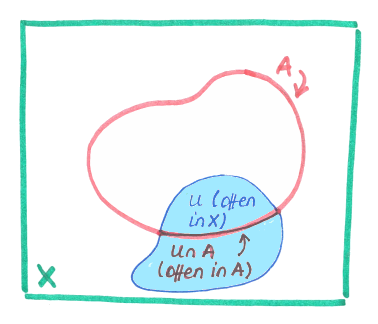
\includegraphics[height=4.5cm]{abb/teilraumtop.png}
        \caption{Teilraumtopologie}
        \label{fig:teilraumtop}
    \end{figure}
    
    
    
    \begin{bsp}[Teilraumtopologie Standardbeispiel]\ \\
        In der Teilraumtopologie von ${\rand A = \{\frac{1}{2^n} \mid n \in \N\} \cup \{0\}}$ (siehe Bsp.~\ref{bsp:standardbsp}) sind alle Mengen $M$ 
        \begin{itemize}
            \item abgeschlossen, die die $0$ enthalten oder für die  $M$ \textit{keine} Häufungspunkte hat.
            \item offen, die die $0$ \textit{nicht} enthalten oder für die $\rand A \setminus M$ \textit{keine} Häufungspunkte hat.
        \end{itemize}
        Dies ist eine einfache Folgerung aus der Eigenschaft von $A$, $0$ als einzigen Häufungspunkt zu haben. 
        Damit sind sowohl ${\HP(M)}$ als auch ${\HP(\rand A \setminus M)}$ ${\{0\}}$ oder $\varnothing$.
        Zusammen mit \\
        ${\cl(M) = M \cup \HP(M)}$ und ${\op(M) = M \setminus \HP(\rand A \setminus M)}$ ergeben sich die Aussagen.
    \end{bsp}


    Analog zu den offenen Mengen entstehen die abgeschlossenen Mengen in $A \subseteq X$ durch Schnitte mit in $X$ abgeschlossenen Mengen.
    %
    \begin{satz} \label{satz:trAbg}\ \vspace{8pt}

        \noindent
        Sei $X$ ein topologischer Raum und $B \subseteq A \subseteq X$. Dann gilt
        \begin{align*}
            B \in \abg_A \quad \quad \Leftrightarrow \quad \quad \exists\: B' \in \abg_X : B = B' \cap A 
        \end{align*}
        (Beweis siehe Anhang \ref{anh:trAbg})
        
    \end{satz}
    %(Beweis siehe \ref{anh:trAbg})


    Ist $A \subseteq X$ offen in $X$, so sind alle in $A$ offenen Mengen auch offen in $X$. Analoges gilt für abgeschlossene Mengen.
    %
    \begin{kor}\label{kor:OX-OA-CX-CA}
        Seien $X$ ein topologischer Raum und $B \subseteq A \subseteq X$. Dann gelten:
        \begin{enumerate}
            \item $A \in \offen_X \to (\: B \in \offen_A \leftrightarrow B \in \offen_X \:)$
            \item $A \in \abg_X \to (\: B \in \abg_A \leftrightarrow B \in \abg_X \:)$
        \end{enumerate}
    \end{kor}
    %
    \begin{bew}\ 
        \begin{enumerate}
            \item Sei $A \in \offen_X$. Falls $B \in \offen_A$ ist, so gibt es ein $U \in \offen_X$ mit $B = U \cap A \in \offen_X$.\\
            Ist andererseits $B \in \offen_X$, so ist $B = A \cap B \in \offen_A$.
            \item Mit vorherigem Satz analog.
        \end{enumerate}
    \end{bew}


    Der folgende Satz wird in den Beweisen von \ref{satz:da1=da2} und \ref{kor:da1=da2} verwendet.
    %
    \begin{satz} \label{satz:dAB<clB}\ \vspace{8pt}

        \noindent
        Seien $X$ ein topologischer Raum und $B \subseteq A \subseteq X$. Dann gilt 
    %
        \begin{align*}
            \rand_A(B) \subseteq \cl_X(B).
        \end{align*}
    %	
        (Beweis siehe Anhang \ref{anh:dAB<clB})
    \end{satz}
%     (Beweis siehe \ref{anh:dAB<clB})


    Der folgende Satz wird zum Beweis von Korollar \ref{kor:cl-rand-A1-A2} verwendet.
    %
    \begin{satz}\label{satz:clA1-teil-clA2}\ \\
        Seien $X$ ein topologischer Raum, ${A_1, A_2 \subseteq X}$ und ${B \subseteq A_1 \cap A_2}$ mit ${\cl_{A_1}(B) \subseteq A_2}$. Dann gilt ${\cl_{A_1}(B) \subseteq \cl_{A_2}(B)}$.\\
        (Beweis siehe Anhang \ref{anh:clA1-teil-clA2})
    \end{satz}
    %
%     (Beweis siehe \ref{anh:clA1-teil-clA2})


    Für einen topologischen Raum $X$ und Teilmengen $A_1, A_2, B \subseteq X$ mit $B \subseteq A_1 \cap A_2$ muss nicht notwendigerweise gelten $\cl_{A_1}(B) \subseteq A_2$.
    %
    \begin{gegenbsp}
        Man nehme $X = \{0,1\}, \offen_X = \{\varnothing, \{0,1\}\}, A_1 = X, A_2 = \{0\}, B = \{0\}$. Dann ist $\abg_X = \{\varnothing, \{0,1\}\}$ also $\abg_{A_1} = \{\varnothing, \{0,1\}\}$ und damit $\cl_{A_1} = \{0,1\} \nsubseteq A_2$
    \end{gegenbsp}
    %
% 		\todo[inline]{FL: müsste es nach ``damit'' heißen:
% 		$\cl_{A_1}(B) = \{0,1\} \nsubseteq A_2$ ?\\
% 		-> BH: das ist richtig}
    %
    Folgender Satz besagt jedoch, dass diese Aussage gilt, falls $A_1$ und $A_2$ Ränder von Mengen sind.
    %
    \begin{satz}\label{satz:cl-dA1-dA2}\ \\
        Seien $X$ ein topologischer Raum, $A_1, A_2 \subseteq X$ und \\
        $B \subseteq \rand A_1 \cap \rand A_2$.
        Dann ist $\cl_{\rand A_1}(B) \subseteq \rand A_2$.\\
        (Beweis siehe Anhang \ref{anh:cl-dA1-dA2})
    \end{satz}
    %
%     (Beweis siehe \ref{anh:cl-dA1-dA2})


    \begin{kor}\label{kor:cl-rand-A1-A2}
        Seien $X$ ein topologischer Raum, $A_1, A_2 \subseteq X$ und $B \subseteq \rand A_1 \cap \rand A_2$.\\
        Dann ist ${\cl_{\rand A_1}(B) = \cl_{\rand A_2}(B)}$.
    \end{kor}
    %
    \begin{bew}
        Aus dem vorherigen Satz folgen $\cl_{\rand A_1}(B) \subseteq \rand_{A_2}B$ und $\cl_{\rand A_2}(B) \subseteq \rand_{A_1}B$. Deshalb lässt sich mit Satz \ref{satz:clA1-teil-clA2} folgern \\
        ${\cl_{\rand A_1}(B) \subseteq \cl_{\rand A_2}(B)}$ und ${\cl_{\rand A_2}(B) \subseteq \cl_{\rand A_1}(B)}$.
    \end{bew}

    Unter den Voraussetzungen von Korollar \ref{kor:cl-rand-A1-A2} gilt nicht notwendigerweise ${\op_{\rand A_1}(B) = \op_{\rand A_2}(B)}$.
    
    \begin{gegenbsp}\label{gegenbsp-teiltop}\ \\
        Als Gegenbeispiel wähle $X = \R^2$, ${A_1 = \{(x,y) \in \R^2 \mid x*y < 0\}}$, ${A_2 = \{(x,y) \in \R^2 \mid x > 0, y > 0\}}$, \\
        ${B = \{0\} \times (0, \infty) \cup (0,\infty) \times \{0\}}$.\\
        Dann ist ${(0,0) \notin \op_{\rand A_1}(B)}$ aber ${(0,0) \in \op_{\rand A_2}(B)}$.
    \end{gegenbsp}
    %
    \begin{figure}[ht]
        \centering
        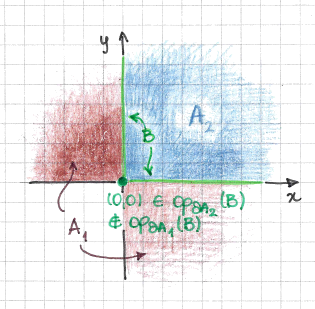
\includegraphics[height=7cm]{abb/gegenbsp-teilraumtop.png}
        \caption{Zu Gegenbeispiel \ref{gegenbsp-teiltop}}
        \label{fig:gegenbsp-teilraumtop}
    \end{figure}

    Daraus folgt, dass sich die Teilraumtopologien auf den Rändern von Mengen unter gewissen Bedingungen ähneln.
    \begin{satz}\label{satz:da1=da2} \ \vspace{8pt}

        \noindent
        Sei $X$ ein topologischer Raum. Seien $A_1, A_2 \subseteq X$ und $B \subseteq A_1 \cap A_2$ so, dass
    %
        \begin{align*}
            \exists\: \, U \in \offen_X: (\: \cl_X(B) \subseteq U \:\land\: U \cap A_1 = U \cap A_2 \:)
        \end{align*}
    %
        gilt. Dann gilt auch  
    %
        \begin{align*}
            \rand_{A_1}(B) = \rand_{A_2}(B).
        \end{align*}
        %
        (Beweis siehe Anhang \ref{anh:da1=da2})
        
    \end{satz}
%     (Beweis siehe \ref{anh:da1=da2})

    %
    \begin{kor}\label{kor:da1=da2} \ \vspace{8pt}

        \noindent
        Sei $X$ ein topologischer Raum. Seien $A_1, A_2 \subseteq X$ und $B \subseteq A_1 \cap A_2$ so, dass
    %
        \begin{align*}
            \exists\: \, U \in \offen_X: (\: \cl_X(B) \subseteq U \:\land\: U \cap A_1 = U \cap A_2 \:)
        \end{align*}
    %
        gilt. Dann gelten auch  
    %
        \begin{enumerate}
            \item \label{kor:da1=da2.1} $\cl_{A_1}(B) = \cl_{A_2}(B)$
            \item \label{kor:da1=da2.2} $\op_{A_1}(B) = \op_{A_2}(B)$
            %\item \label{kor:da1=da2.3} $\co_{A_1}(B) = \co_{A_2}(B)$
            %\item \label{kor:da1=da2.4} $\oc_{A_1}(B) = \oc_{A_2}(B)$
        \end{enumerate} 
        (Beweis siehe Anhang \ref{anh:kor.da1=da2})
    \end{kor}
%     (Beweis siehe Anhang \ref{anh:kor.da1=da2})
    %\todo[inline]{3 und 4 auslagern, da co und oc noch nicht eingeführt sind}
    
    
    
    
    
    
                    %%%%%%%%%%%%%%%%%%%%%%%%%%%%%%%%%%%%%%
                    %%%                                %%%
%%%%%%%%%%%%%%%%%%%%%%%   Topologie metrischer Räume   %%%%%%%%%%%%%%%%%%%%%%%%%%%%%
                    %%%                                %%%
                    %%%%%%%%%%%%%%%%%%%%%%%%%%%%%%%%%%%%%%


\section{Topologie metrischer Räume}\label{sec:top-metr-raeume}

    Der hier vorgestellte Interpretationsansatz arbeitet mit Teilmengen des $\R^3$ und nutzt die topologische Struktur, die dieser Raum durch seine Metrik mit sich bringt.
    In diesem Abschnitt geht es darum, wie Metriken -- insbesondere die euklidische Metrik auf $\R^n$ -- Topologien erzeugen.
    
    Ein
    \marginpar{metrischer Raum}
    metrischer Raum ist eine Menge mit einer Metrik, also einer Abbildung, die anschaulich gesprochen je zwei Punkten ihren Abstand zuordnet.
    %
    \begin{dfn}[Metrischer Raum]\label{def:metr}\ \vspace{8pt}

        \noindent
        Ein \thmemph{metrischer Raum} ist ein Paar $(X,d)$ bestehend aus
    %
        \begin{itemize}
            \item einer Menge $X$ (\thmemph{Grundmenge}) und
            \item einer Abbildung $ d: X^2 \rightarrow \R_0^+$ (\thmemph{Metrik})
        \end{itemize}
    %
        so dass für alle $x$, $y$ und $z$ aus $X$ gelten
    %
        \begin{enumerate}
            \item $d(x,y) = 0 \quad \quad \Leftrightarrow \quad \quad x=y \qquad$ (positive Definitheit) 
            \item $d(x,y) = d(y,x) \qquad$ (Symmetrie)
            \item $d(x,y) + d(y,z) \geq d(x,z) \qquad$ (Dreiecksungleichung)
        \end{enumerate}
    %	
    \end{dfn}


    Die
    \marginpar{$\varepsilon$-Umgebung}
    $\varepsilon$-Umgebung eines Punktes besteht aus allen Punkten, die ihm $\varepsilon$-nahe sind, also einen kleineren Abstand als $\varepsilon$ haben.
% 		\todo[inline]{Zwei Quellen, in denen ich geschaut habe, nehmen dem Satz hierüber
% 		entsprechend $d(x,y) < \varepsilon$ in der Definition, statt $\leq$ darin. ``(offene)'' Umgebung würde auch dazu passen. Ich bin mir dennoch nicht 100\% sicher, was Du haben willst, daher als Kommentar.\\
% 		-> BH: <}
    %
    \begin{dfn}[$\varepsilon$-Umgebung]\label{def:eps-umg}\ \vspace{8pt}

        \noindent
        Seien (X,d) ein metrischer Raum, $x \in X$, $\varepsilon > 0$. Dann ist
        \begin{align*}
            \ball_\varepsilon(x) := \{y \in X \mid d(x,y) < \varepsilon \}
        \end{align*}
        die (offene) \thmemph{$\varepsilon$-Umgebung} von $x$.
        
    \end{dfn}


    In
    \marginpar{Topologie metrischer Räume}
    einem metrischen Raum ist ein innerer Punkt einer Menge ein Punkt, der eine $\varepsilon$-Umgebung hat, die ganz in dieser Menge liegt. Dies führt zu folgender Definition für offene Mengen in metrischen Räumen.
    \begin{dfn}[Topologie metrischer Räume] \label{def:topMet} \ \vspace{8pt}

        \noindent
        Sei $(X,d)$ ein metrischer Raum. Dann ist
        \begin{align*}
            \offen_d := \{A \subseteq X \mid \forall\: a \in A \; \exists\: \varepsilon > 0: \ball_\varepsilon(a) \subseteq A \}
        \end{align*}
        die von \thmemph{$d$ induzierte Topologie} auf $X$.
        
    \end{dfn}

    Der folgende Satz besagt, dass das so definierte Mengensystem tatsächlich im Sinne von \ref{def:top} eine Topologie ist.
    %
    \begin{satz}
        Sei $(X,d)$ ein metrischer Raum. Dann ist $(X,\offen_d)$ ein topologischer Raum.
    \end{satz}
    %
    Der Beweis ist einfach und ist unter anderem in [\cite{manetti-m-2015--a}] zu finden (Definition 3.4).

    Die topologischen Symbole einer durch eine Metrik $d$ induzierten Topologie kennzeichnen wir durch ein tiefgestelltes $d$.
    %
    \begin{nota} \ \vspace{8pt}

        \noindent
        Sei $(X,d)$ ein metrischer Raum. Wir bezeichnen 
        \begin{itemize}
        \item die \thmemph{Menge der abgeschlossenen Mengen} in $X$ mit $\abg_d$
        \item den \thmemph{Kernoperator} in $X$ mit $\op_d$
        \item den \thmemph{Abschlussoperator} in $X$ mit $\cl_d$
        \item den \thmemph{Randoperator} in $X$ mit $\rand_d$
        %\item den $oc$-Operator in $X$ mit $oc_d$
        %\item den $co$-Operator in $X$ mit $co_d$
        \end{itemize}
    \end{nota}


    Die abgeschlossenen Mengen in einem metrischen Raum lassen sich auf ähnliche Weise definieren wie die offenen.
    %
    \begin{satz} \label{satz:Cd} \ \hspace{8pt}

        \noindent
        Sei $(X,d)$ ein metrischer Raum. Dann gilt
        \begin{align*}
            \abg_d := \{A \subseteq X \mid \forall\: x \in X (\: \forall\: \varepsilon > 0 : \ball_\varepsilon \cap A \neq \varnothing \rightarrow x \in A \:) \}
        \end{align*}
        
    \end{satz}
    %
    \begin{bew}
        \begin{align*}
            &\abg_d = \{A \subseteq X \mid X \setminus A \in \offen_d\} \\
            &= \{A \subseteq X \mid \forall\: x \in X \setminus A \; \exists\: \varepsilon > 0 : \ball_\varepsilon(x) \subseteq X \setminus A\} \\
            &= \{A \subseteq X \mid \forall\: x \in X (\: x \notin A \rightarrow \exists\: \varepsilon > 0 : \ball_\varepsilon(x) \cap A = \varnothing \:) \} \\
            &= \{A \subseteq X \mid \forall\: x \in X (\: \forall\: \varepsilon > 0 : \ball_\varepsilon(x) \cap A \neq \varnothing \rightarrow x \in A \:) \} 
        \end{align*}
    \end{bew}


%     \begin{satz} \label{satz:dAabg}
%         Seien $(X,d)$ ein metrischer Raum, $A \subseteq X$. Dann gilt $\rand_d A \in \abg_d$.
%     \end{satz}
%     (Beweis siehe \ref{anh:dAabg})
      % bem: unnötig, da schon in Korollar \ref{kor:rand-abg} allgemein bewiesen


%     \begin{kor} \label{kor:BinCA-BinC}
%         Seien $(X,d)$ ein metrischer Raum, $A \subseteq X$, $B \in \abg_{\rand_d A}$. Dann gilt: $B \in \abg_d$.
%     \end{kor}
%     %
%     \begin{bew}
%         Aus Korollar \ref{kor:rand-abg} folgt $\rand_d A \in \abg$. Aus Satz \ref{satz:trAbg} wissen wir da $B \in \abg_{\rand_d A}$ ist gibt es ein $B' \in \abg_d$ mit $B = B' \cap \rand_d A$. Als Schnitt abgeschlossener Mengen ist dann $B$ auch abgeschlossen (vgl. Satz \ref{satz:cl}).
%     \end{bew}
    % bem: unnötig, da Spezialfall von Korollar \ref{kor:OX-OA-CX-CA}


    \todo[inline]{prüfen, ob folgender Satz raus kann, da er nicht verwendet wird}
    \begin{satz}\label{satz:ball}
    Sei $(X,d)$ ein metrischer Raum, $x \in X$. Seien $\varepsilon, \delta \in \R$ mit $0 < \varepsilon< \delta$. Dann gilt: $\cl_d(\ball_\varepsilon(x)) \subseteq \ball_\delta(x)$.
    \end{satz}
    %
    \begin{bew}
    Sei $y \in \cl_d(\ball_\varepsilon(x))$. Dann gilt für alle $\eta > 0$:\\ $\ball_\eta(y) \cap U_\varepsilon(x) \neq \varnothing$. Sei $\eta = \delta - \varepsilon$. Sei $z \in U_\eta(y) \cap U_\varepsilon(x)$. Nach der Dreiecksungleichung gilt dann:
    $$d(x,y) \leq d(x,z) + d(z,y) < \varepsilon + \eta = \delta.$$
    Also ist $y \in \ball_\delta(x)$.
    \end{bew}


    Auf
    \marginpar{Standardmetrik des $\R^n$}
    $\R^n$ liefert der euklidische Abstand, der mit Hilfe des Skalarprodukts berechnet werden kann, eine Metrik -- die sogennannte Standardmetrik des $\R^n$.
    %
    \begin{dfn}[Standardmetrik des $\R^n$]\label{def:standardmetrik}\ \vspace{8pt}

        \noindent
        Auf $\R^n$ ist die \thmemph{Standardmetrik} $d_n : \R^n \times \R^n \rightarrow \R_0^+$ definiert durch
        \begin{align*}
            d_n(x,y) = \sqrt{(x-y)^2}
        \end{align*}
        
        \noindent
        Die durch die Standardmetrik induzierte Topologie auf $\R^n$ bezeichnen wir mit $\offen_n$.
        
    \end{dfn}

    \begin{konv}\label{konv:d3}
        Statt $d_3$ schreiben wir auch einfach $d$.	
    \end{konv}
    
    \begin{bem}
        Die durch die Standardmetrik induzierte Topologie auf $\R$ stimmt mit der in Bsp.~\ref{bsp:standard-r} definierten Standardtopologie überein.
    \end{bem}
%
%
    Der folgende Satz besagt, dass ein stetiger Weg, der in einer Menge beginnt und außerhalb von ihr endet, immer einen Randpunkt passieren muss. Er wird zum Beweis von Satz \ref{satz:r2} verwendet und lässt sich möglicherweise nutzen, um zu zeigen, dass gewisse Punkte äußere Randpunkte sind (zum Begriff des äußeren Randes siehe Abschnitt \ref{sec:aeusserer-rand}).
    %
    \begin{satz}\label{satz:weg} %verwendung: {satz:r2}
        Sei $X$ ein topologischer Raum. Sei $A \subset X$. Seien $x \in A$, $y \in X \setminus A$. Seien $a,b \in \mathbb{R}$ mit $a < b$. Sei $\gamma : [a,b] \to X$ ein stetiger Weg mit $\gamma(a) = x$ und $\gamma(b) = y$. Dann gibt es ein $t \in [a,b]$ mit $\gamma(t) \in \rand A$.
    \end{satz}
    
    \begin{figure}[ht]
        \centering
        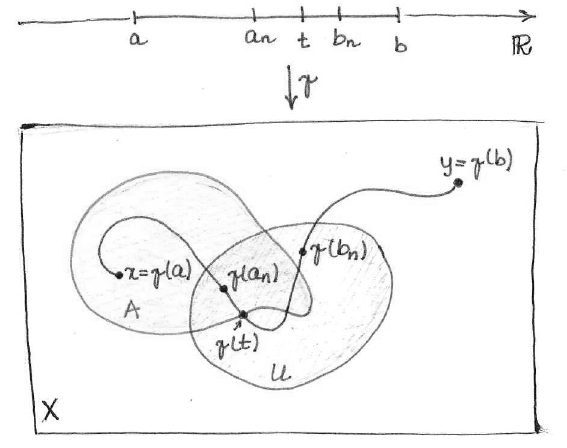
\includegraphics[height=5cm]{abb/weg_sw.png}
        \caption{Zum Beweis von Satz \ref{satz:weg}}
        \label{fig:weg}
    \end{figure}

    \begin{bew}
        Definiere eine Intervallschachtelung $([a_i, b_i])_{i \in \N}$ auf folgende Weise:
        \begin{enumerate}
            \item $a_0 = a, b_0 = b$
            \item Wenn $\gamma(\frac{a_i + b_i}{2}) \in A$, so setze $a_{i+1} = \frac{a_i + b_i}{2}$, $b_{i+1} = b_i$\\
            Ansonsten setze $a_{i+1} = a_i$, $b_{i+1} = \frac{a_i + b_i}{2}$
        \end{enumerate}
        Sei $t$ die eindeutige reelle Zahl, die in allen Intervallen $[a_i, b_i]$ enthalten ist.\\
        Behauptung: Dann ist $\gamma(t) \in \rand A$.\\
        Beweis der Behauptung: Zu zeigen ist: 
        \[\forall\: U \in \offen_X: (\: \gamma(t) \in U \rightarrow (\: U \cap A \neq \varnothing \:\land\: U \setminus A \neq \varnothing \:) \:).\]
        Nach Konstruktion der Intervallschachtelung gelten:
        \begin{enumerate}
        \item $\forall\: \varepsilon > 0\ \exists\: n \in \N\ \forall\: i \geq n: \ball¸_\varepsilon(t) \subseteq [a_i,b_i]$
        \item $\forall\: i \in \N : (\: \gamma(a_i) \in A \:\land\: \gamma(b_i) \notin A \:)$
        \end{enumerate}
        Sei nun ${U \in \offen_X}$. Da $\gamma$ stetig ist, ist ${\gamma^{-1}(U) \in \offen_{\R}}$. Da ${t \in \gamma^{-1}(U)}$ ist, gibt es also ein ${\varepsilon > 0}$ mit ${\ball_\varepsilon(t) \subseteq \gamma^{-1}(U)}$.\\
        Sei ${n \in \N}$ mit ${[a_i, b_i] \subseteq \ball_\varepsilon(t)}$ für alle ${i \geq n}$, dann sind \\
        ${\gamma(a_n) \in U \cap A}$ und ${\gamma(b_n) \in U \setminus A}$.
    \end{bew}
